\subsubsection{Эмбеддинговая система и роутер}
\label{sec:emb_sys_and_router}

Основным итогом настоящего исследования стало создание двух ключевых компонентов: гибкой эмбеддинговой подсистемы
и обучаемого роутера для блока MoTE. Эти наработки не только обеспечивают надёжный фундамент для дальнейшего
развития FinABYSS, но и открывают широкий простор для применения в смежных прикладных проектах.

В рамках исследования мы провели серию экспериментов по отбору оптимальных комбинаций эмбеддинговых моделей,
методов понижения размерности и алгоритмов кластеризации, используя разные метрики для настройки гиперпараметров.
На первом этапе базовая цепочка состояла из ModernBERT, UMAP (косинусная метрика), HDBSCAN (эвклидова метрика)
оптимизировалась по коэффициенту силуэта. Несмотря на удовлетворительные результаты, мы отметили сильную
зависимость от структуры кластеров и чувствительность силуэта к форме кластеров.

Второй этап повторил ту же связку, но в качестве целевой метрики был выбран DBCV-индекс. Благодаря свойству
DBCV учитывать плотностные особенности и неоднородность распределения точек, гиперпараметры, подобранные
под DBCV, обеспечили более семантически согласованные и плотные кластеры.

Наконец, мы протестировали тонко настроенную на задачу STS версию ModernBERT ('gte-modernbert-base') \parencite{Warner2024ModernBERT, MGTE2024} в сочетании с UMAP,
но уже с $L_2$–эвклидовой метрикой, и тем же HDBSCAN, также настроенным под $L_2$–евклидову дистанцию (Таблица \ref{tab:experiment_configs}).
днако это сочетание уступило предыдущему: полученный DBCV-индекс составил лишь 0.405 против 0.476 у пары "cosine + euclidean" (Таблица \ref{tab:experiment_results}).

\begin{longtable}[c]{|l|ll|}
    \caption{Description of the final configurations of experiments conducted on a subsample of 10,000 embeddings.}
    \label{tab:experiment_configs}\\
    \hline
    \multicolumn{1}{|c|}{\multirow{2}{*}{\textbf{Model}}} & \multicolumn{2}{c|}{\textbf{Configuration}}                         \\ \cline{2-3}
    \multicolumn{1}{|c|}{}                                 & \multicolumn{1}{c|}{(I)}               & \multicolumn{1}{c|}{(II)}  \\ \hline
    \endfirsthead

    \endhead

    UMAP    & \multicolumn{1}{l|}{$L_2$-Euclidean} & \multicolumn{1}{l|}{Cosine}    \\
    HDBSCAN & \multicolumn{1}{l|}{$L_2$-Euclidean} & \multicolumn{1}{l|}{Euclidean} \\ \hline
\end{longtable}

Дополнительный анализ шумовых точек и структуры кластеров не подтвердил это преимущество (Таблица \ref{tab:experiment_results}),
однако в ходе анализа выяснилось, что подобная ситуация просиъодит по причине внутренней нестрабильности GPU реализации \parencite{cuml2020machine}. На метрике же,
данный факт не сказался существенно негативным образом. При использовании $L_2$–метрики
доля шумовых точек достигала 39.54\%, число кластеров --- 73 (при максимальном размере 3 824 точек и минимальном --- 365).
Для пары "cosine + euclidean" больше точек было отмечено как шум 43.38\%, а число кластеров увеличилось до 141; при этом максимальный
кластер вырос до 2 558 точек, а минимальный сократился до 147. Так как целевая метрика именно DBCV, можно сделать вывод, что
подход "cosine + euclidean" продемонстрировал лучшую устойчивость кластеров.

% Please add the following required packages to your document preamble:
% \usepackage{multirow}
% \usepackage{longtable}
\begin{table}[!htbp]
\begin{longtable}[c]{|cl|cc|}
    \caption{Summary table of the results of hyperparameter optimization performed for three specified configurations on a subsample of 10,000 embeddings.}
    \label{tab:experiment_results}\\
    \hline
    \multicolumn{2}{|c|}{\multirow{2}{*}{\textbf{Best trial}}} & \multicolumn{2}{c|}{\textbf{Configuration}}                                                \\ \cline{3-4}
    \multicolumn{2}{|c|}{}                                     & \multicolumn{1}{c|}{(I)} & \multicolumn{1}{c|}{(II)} \\ \hline
    \endfirsthead

    \endhead

    \hline
    \endfoot

    \endlastfoot

    \multicolumn{1}{|c|}{\multirow{7}{*}{\textbf{Hyperparameters}}} & n\_components            & \multicolumn{1}{c|}{47}                & \multicolumn{1}{c|}{41}             \\
    \multicolumn{1}{|c|}{}                                          & n\_neighbors             & \multicolumn{1}{c|}{70}                & \multicolumn{1}{c|}{75}             \\
    \multicolumn{1}{|c|}{}                                          & min\_dist                & \multicolumn{1}{c|}{0,0}               & \multicolumn{1}{c|}{0,065}          \\
    \multicolumn{1}{|c|}{}                                          & spread                   & \multicolumn{1}{c|}{6,5}               & \multicolumn{1}{c|}{6,4}            \\
    \multicolumn{1}{|c|}{}                                          & negative\_sample\_rate   & \multicolumn{1}{c|}{10}                & \multicolumn{1}{c|}{11}             \\
    \multicolumn{1}{|c|}{}                                          & min\_cluster\_size       & \multicolumn{1}{c|}{360}               & \multicolumn{1}{c|}{145}            \\
    \multicolumn{1}{|c|}{}                                          & min\_samples             & \multicolumn{1}{c|}{180}               & \multicolumn{1}{c|}{170}            \\ \hline
    \multicolumn{1}{|c|}{\multirow{5}{*}{\textbf{Statistics}}}      & Max cluster size         & \multicolumn{1}{c|}{3824}              & \multicolumn{1}{c|}{2558}           \\
    \multicolumn{1}{|c|}{}                                          & Min cluster size         & \multicolumn{1}{c|}{365}               & \multicolumn{1}{c|}{147}            \\
    \multicolumn{1}{|c|}{}                                          & Total clusters           & \multicolumn{1}{c|}{73}                & \multicolumn{1}{c|}{141}            \\
    \multicolumn{1}{|c|}{}                                          & Noise \%                 & \multicolumn{1}{c|}{\textbf{39,54\%}}  & \multicolumn{1}{c|}{43,38\%}        \\
    \multicolumn{1}{|c|}{}                                          & DBCV Index               & \multicolumn{1}{c|}{0,397}             & \multicolumn{1}{c|}{\textbf{0,407}} \\ \hline
\end{longtable}
\end{table}

Экспериментальные результаты однозначно свидетельствуют о превосходстве схемы ModernBERT + UMAP
с косинусной метрикой и HDBSCAN с эвклидовой дистанцией в задачах тематической кластеризации
финансовых текстов. В сочетании с оптимизацией по DBCV-индексу данный подход формирует наиболее
семантически связные группы, минимизирует долю шумовых экземпляров и предоставляет более стабильную
основу для последующего обучения роутера MoTE.

Тем не менее, к сожалению, были выявлены и явные проблемные места текущей реализации.
Полученные кластеры и их структура не могут инкрементально обновляться при потоковых
поступлениях новых публикаций, что происходит по нескольким причинам. Во-первых, обученная
модель является GPU-реализацией из библиотеке 'cuML', в которой лишь после проведения исследования
были обнаружены критические ошибки в коде версии 25.02 \parencite{cuml2020machine}. Во-вторых, выбранный
алгоритм UMAP достаточно плохо работает в инкрементальном режиме по своей природе, именно
поэтому существуют другие реализации, как например AlignedUMAP \parencite{mcinnes2018umap-software}
или ParametricUMAP, основанный на нейронной сети в качестве базовой модели \parencite{ParametricUMAP2020}.
К сожалению, обе данные реализации доступны исключительно для обучения на центральном, а не графическом процессоре.
А для обучения на центральном процессоре в контексте текущего исследования недостаточно вычислительных ресурсов.

Таким образом, узким местом данного исследования и предложенного решения является недостаток вычислительных
мощностей для обучения моделей, что будет доработано в дальнейших исследованиях.

\subsubsection{Семантическая карта}

Наконец, на базе разработанной эмбеддинговой подсистемы и роутера MoTE была обучена отдельная модель UMAP,
призванная переводить векторы из промежуточного латентного пространства кластеризации в двумерное представление,
удобное для визуального анализа. Именно эта проекция лежит в основе Семантической карты финансовых публикаций ---
одного из ключевых компонентов интерфейса FinABYSS, обеспечивающего глубокое и интуитивно понятное исследование
тематической структуры новостных потоков.

\begin{figure}[H]
    \centering
    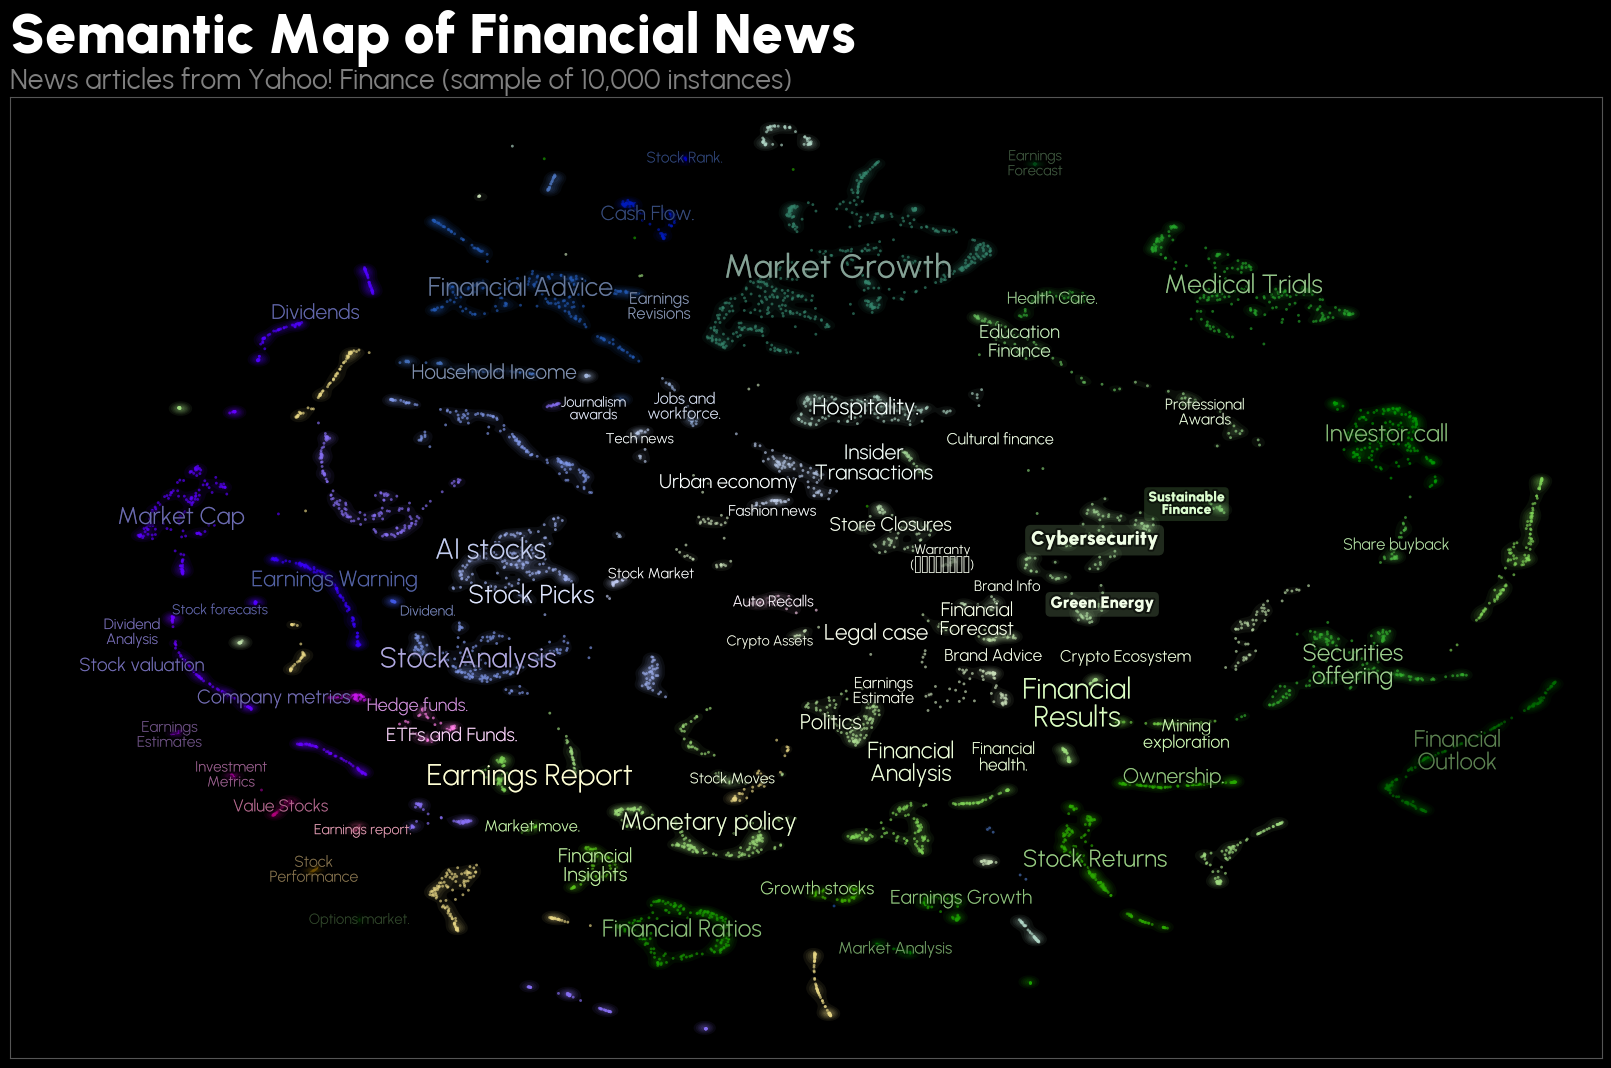
\includegraphics[width=1\linewidth]{img/semantic_map.png}
    \caption{Статичная емантическая карта, разработанная на основе подвыборки из 10 000 финансовых публикаций,
    опубликованных в период с 17.09.2023 по 18.04.2025, и кластеризованных по темам.}
    \label{fig:semantic_map}
\end{figure}

Для начала была реализована статическая версия карты, на которой отображены 100000 финансовых статей периода
с сентября 2023 по март 2025 года, разбитые на кластеры по тематике (Изображение \ref{fig:semantic_map}).
Каждый кластер промаркирован автоматически сгенерированным словом-меткой без какой-либо ручной аннотации.
Несмотря на автоматический характер присвоения, метки получились репрезентативными: плотные группы статей,
посвящённые здравоохранению, «Устойчивым финансам», «Кибербезопасности» и «Зелёной энергетике», расположены
рядом, что отражает их семантическую близость; аналогично происходит с кластерами «Политика» и «Монетарная политика».

Однако статическая карта демонстрирует потенциал лишь UMAP-проекции. Интерактивная Семантическая
карта FinABYSS выходит далеко за рамки простой визуализации точек:

\begin{itemize}
    \item Наведение курсора на любую точку раскрывает метаданные статьи: заголовок, дата и время публикации,
    иерархическую тему (макро–/мезо–/микротема), автора и источник. При этом доступен предпросмотр полного
    текста и прямая ссылка на оригинал публикации.
    \item Механизм поиска по ключевым словам позволяет быстро отфильтровать статьи, содержащие специальные термины.
    Поиск можно комбинировать с фильтрами по диапазону дат, объёму публикаций и другим числовым признакам (например,
    объёму текста или количеству просмотров), что облегчает точечное обнаружение исторических событий и триггеров
    на графике.
    \item Раздел источники и темы даёт возможность включать и исключать источники новостей или целевые кластеры,
    помогая сфокусироваться на релевантных публикациях в сложных аналитических сценариях.
    \item Также для статей доступна функция облака слов, формируемого на основе наиболее частых слов, встречающихся
    в выделанной группе текстов. Облако слов мгновенно отображает доминирующие термины и паттерны обсуждения,
    что дополняет количественную канву графика качественными характеристиками.
\end{itemize}

Таким образом, Семантическая карта FinABYSS представляет собой полноценную аналитическую систему,
объединяющую мощь выбранных моделей UMAP и HDBSCAN, а при дальнейшем развитии и гибридной CNN-LSTM-архитектуры
и MoE-подхода к оценке тональностей. Она обеспечивает исследователю возможность не только визуально различать
именованные кластеры и их взаимное расположение, но и глубоко погружаться в содержание каждой публикации,
комбинируя автоматические и ручные методы анализа.

Разработанная интерактивная Семантическая карта выступает естественным продолжением предыдущих модулей FinABYSS.
Все звенья конвейера связаны в единую цепь. Инструмент предлагает пользователю прозрачный, масштабируемый
и гибко настраиваемый интерфейс для семантического исследования финансовых новостей, где каждый элемент ---
от кластерных меток до облака слов — отражает результаты вычислительной логики системы и поддерживает экспертные
решения при анализе рыночных процессов.

\subsubsection{Динамическое тематическое моделирование}

Помимо семантической карты, FinABYSS предоставляет мощный инструментарий для анализа лингвистических
особенностей сформированных тематических групп и динамического темпорального моделирования тем.
Все входящие тексты проходят описанный в \hyperref[sec:sys_dev]{Разделе 2.4} пайплайн постобработки в контексте Аналитического
GUI (см. \hyperref[sec:sys_dev]{Раздел 3.1.6}), где каждому документу присваивается превалирующая тема,
а затем извлекаются и агрегируются соответствующие лексические признаки.

Так, система визуализирует частотное распределение самых релевантных слов в рамках выбранной темы
(Изображение \ref{fig:topics_words_freqs}). Такая лингвистическая панель служит двум целям:

\begin{itemize}
    \item Во-первых, это позволяет после разработки системы в ручном режиме провалидировать качество сформированных
    тем и оценить насколько они уникальны и семантически однородны.
    \item Во-вторых, эта функциональность может быть весьма полезна при первичном знакомстве финансового аналитика
    с системой. Финансовый аналитик, впервые работающий с FinABYSS, получает мгновенное представление о содержании каждой темы без глубокого чтения текстов.
\end{itemize}

Именно последний факт послужил причиной включения данной функциональности в набор основных инструменты GUI.

\begin{figure}[H]
    \centering
    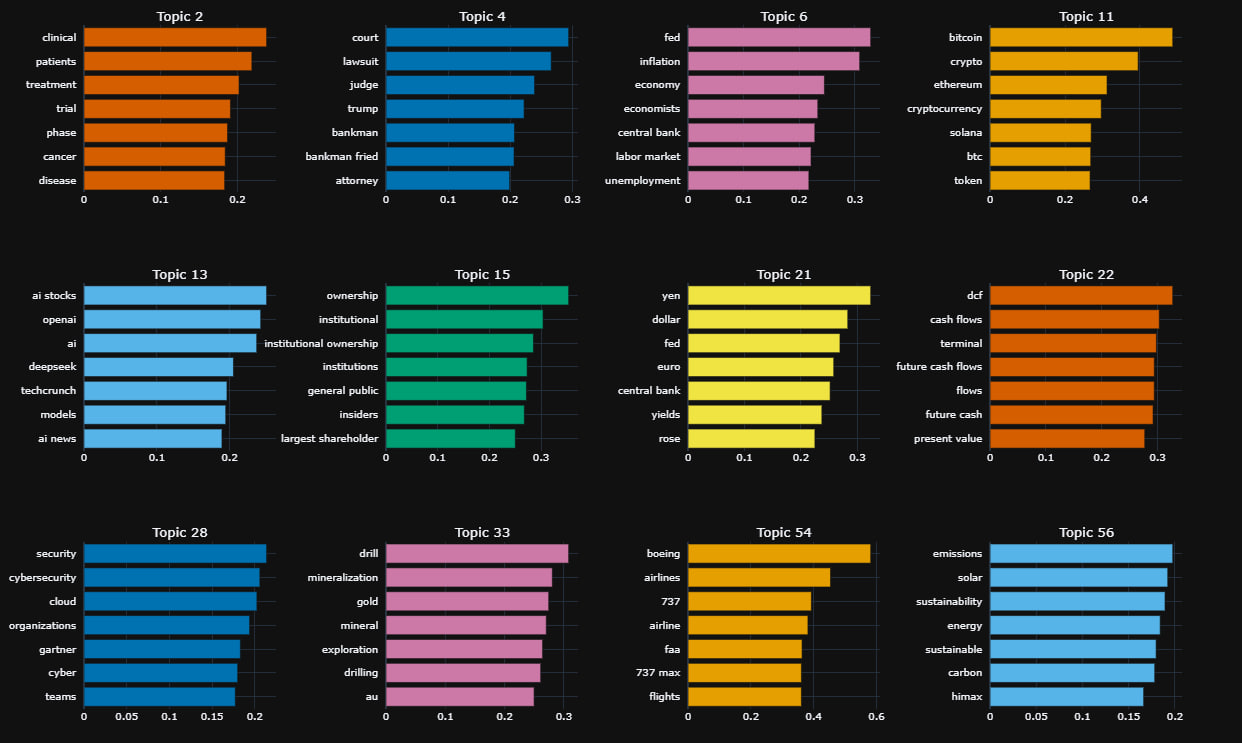
\includegraphics[width=1\linewidth]{img/topics_words_freqs.png}
    \caption{Ранжированные по релевантности термины выборки из 12 тем.}
    \label{fig:topics_words_freqs}
\end{figure}

Для иллюстрации данного функционала случайным образом была сформирована выборка из
125 000 публикаций и внутри них было выбрано 12 тем для отображения. Среди выборки
все темы несомненно несут прикладное значение для финансовых рынков. Причем есть
более общие отраслевые темы, такие как:

\begin{itemize}
    \item Тема №2, связанная с фармацевтической отраслью;
    \item Тема №13, связанная с сектором искуственного интеллекта;
    \item Тема №28, связанная с кибербезопасностью;
    \item Тема №33, связанная с горнодобывающей отраслью;
    \item Тема №54, связанная с авиационной промышленностью.
\end{itemize}

С другой стороны в выборку попала и общая тема, которая стоит на повестке дня и в финансах ---
Тема №56, которая явно относится к ESG. Наконец, есть и узкоспециализированные финансовые темы,
которые также были выявлены автоматически:

\begin{itemize}
    \item Тема №4, связанная с судебными процессами и разбирательствами, которая потенциально
    является крайне важной и влиятельной в контексте ценообразования стоимости актива;
    \item Тема №6, связанная с внешнеэкономическими факторами и экономикой, в общем;
    \item Тема №11, напрямую связанная с рынком активов, а именно криптовалют;
    \item Тема №15, связанная с правами собственности на компании;
    \item Тема №21, связанная с валютным рынком;
    \item Тема №22, связанная с денежными потоками, включая будущие, настоящие и дисконтированные денежные потоки.
\end{itemize}

Так, мы можем наблюдать за лингвистическими особенностями тематических групп,
а также крайне быстро и эффективно изучать как различия между ними, так и конкретные темы вглубь.

С другой стороны, было бы крайне полезно понимать как темы меняются сквозь время, ведь информационное медиапространство
крайне нестабильно, а повестка дня в современном обществе меняется крайне быстро. Так, FinABYSS реализует
динамическое тематическое моделирование через интерактивный график тематических временных рядов.

\begin{figure}[H]
    \centering
    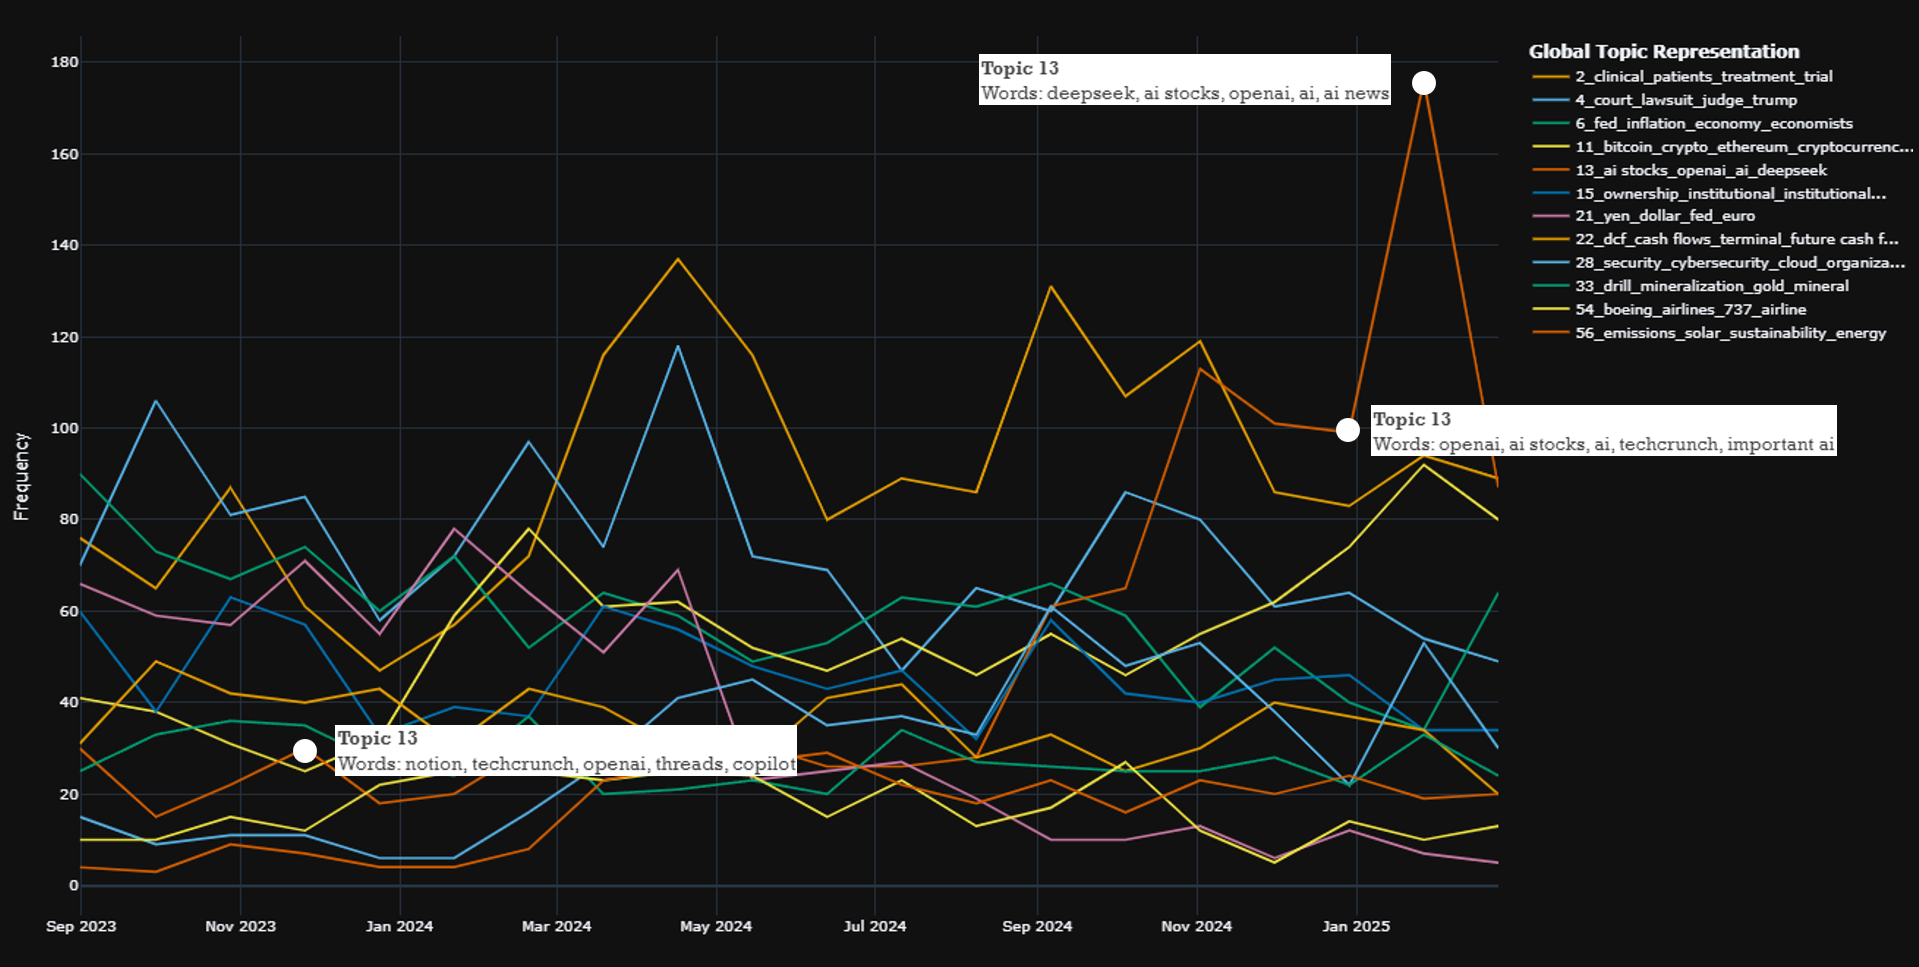
\includegraphics[width=1\linewidth]{img/dynamic_topic_modeling.png}
    \caption{Эволюционное тематическое моделирование и наиболее релевантные термины выборки из 12 тем за период с 17.09.2023 по 18.04.2025.}
    \label{fig:dtm}
\end{figure}

На Изображении \ref{fig:dtm} представлена та же выборка из 12 тем. Ось абсцисс отражает интервал публикаций (настраиваемый:
от дневного до месячного или годового), ось ординат --- число статей по каждой теме за соответствующий период. При наведении
курсора выводятся пять наиболее репрезентативных слов, характеризующих тему в данном временном окне. Пользователь может
изменить число отображаемых слов.

Преимущества такого подхода очевидны:

\begin{itemize}
    \item Раннее обнаружение трендов. Аналитик может наблюдать за появлением новых лексических маркеров
    или ростом публикационной активности в тематических группах, что служит сигналом зарождающихся событий.
    \item Отслеживание циклических явлений. Так, для Темы 13 (ИИ) на графике и в декабре 2023 года,
    и в декабре 2024 года появляется слово TechCrunch — название одной из крупнейших и самых престижных
    конференций в сферах IT и AI. Ежегодно конференция выпускает множество крупнейших стартапов, которые
    в дальнейшем получают крупное финансирования. Таким образом, имея данную визуализацию, аналитик может
    меньшими усилиями оставаться в курсе значимых для финансов циклических событий.
    \item Реакция на форс-мажорные события. В феврале 2025 по той же Теме 13 наблюдается резкий пик из-за
    нонса китайской LLM DeepSeek R1. Этот инцидент крайне важен, так как в последствии он стал причиной обрушения
    акций Nvidia, крупнейшей компании поставляющей вычислительное оборудование.
\end{itemize}

Таким образом, FinABYSS не ограничивается статическим построением тематических кластеров:
взаимодействие с лингвистическими метриками и темпоральными трендами превращает систему
в универсальную платформу для финансовой аналитики. Эксперт может переходить от макро-трендов
к микро-лексическим деталям в несколько кликов, комбинировать фильтры по дате, источнику и тематике,
изучать эволюцию терминологии и оперативно реагировать на появление новых ключевых слов или аномальное
изменение частот. Это делает FinABYSS не просто инструментом кластеризации, а полноценной экосистемой
для семантического мониторинга и прогнозирования воздействия медийных сигналов на динамику финансовых
активов.

\subsubsection{Прикладное значение}
\label{sec:practical_importance}

Подводя итоги, стоит подчеркнуть, что разработанная система FinABYSS представляет собой не просто набор моделей,
а полноценный инструмент для оперативного обнаружения критических сигналов на финансовых рынках. Семантическая
карта, глубокая тематическая кластеризация и временные ряды новостей позволяют финансовому аналитику мгновенно
реагировать на неожиданные события, снижать риски и извлекать прибыль.

Так, рассматривая исключительно функциональность Семантической Карты, можно найти несколько критически важных
событий, которые сразу же после попадания в сеть своевременно отразились в тематическом кластере «Судебные
разбирательства».

Так, первый иллюстративный пример (Изображение \ref{fig:citi_group}) демонстрирует, как статья от 22 мая 2024 года
повлияла на стоимость акций целевой компании. Данная новость осветила скандал с обвалом стоимости европейских акций
по причине недостаточного контроля за трейдинговыми операциями со стороны одного из 4 крупнейших банков в мире ---
Citi Group (C.NYSE) — акции которого торгуются на Нью-Йоркской фондовой бирже. После данной новости, которая так же
сообщала о назначении рекордного штрафа банку со стороны британского правительства, за ближайшие 28 часов акции компании
упали почти на 4\%. В последующие 23 дня, пока шли судебные разбирательства, появлялись дополнительные репортажи
и происходила отложенная рыночная реакция, цена уменьшилась почти на 10\%.

\begin{figure}[H]
    \centering
    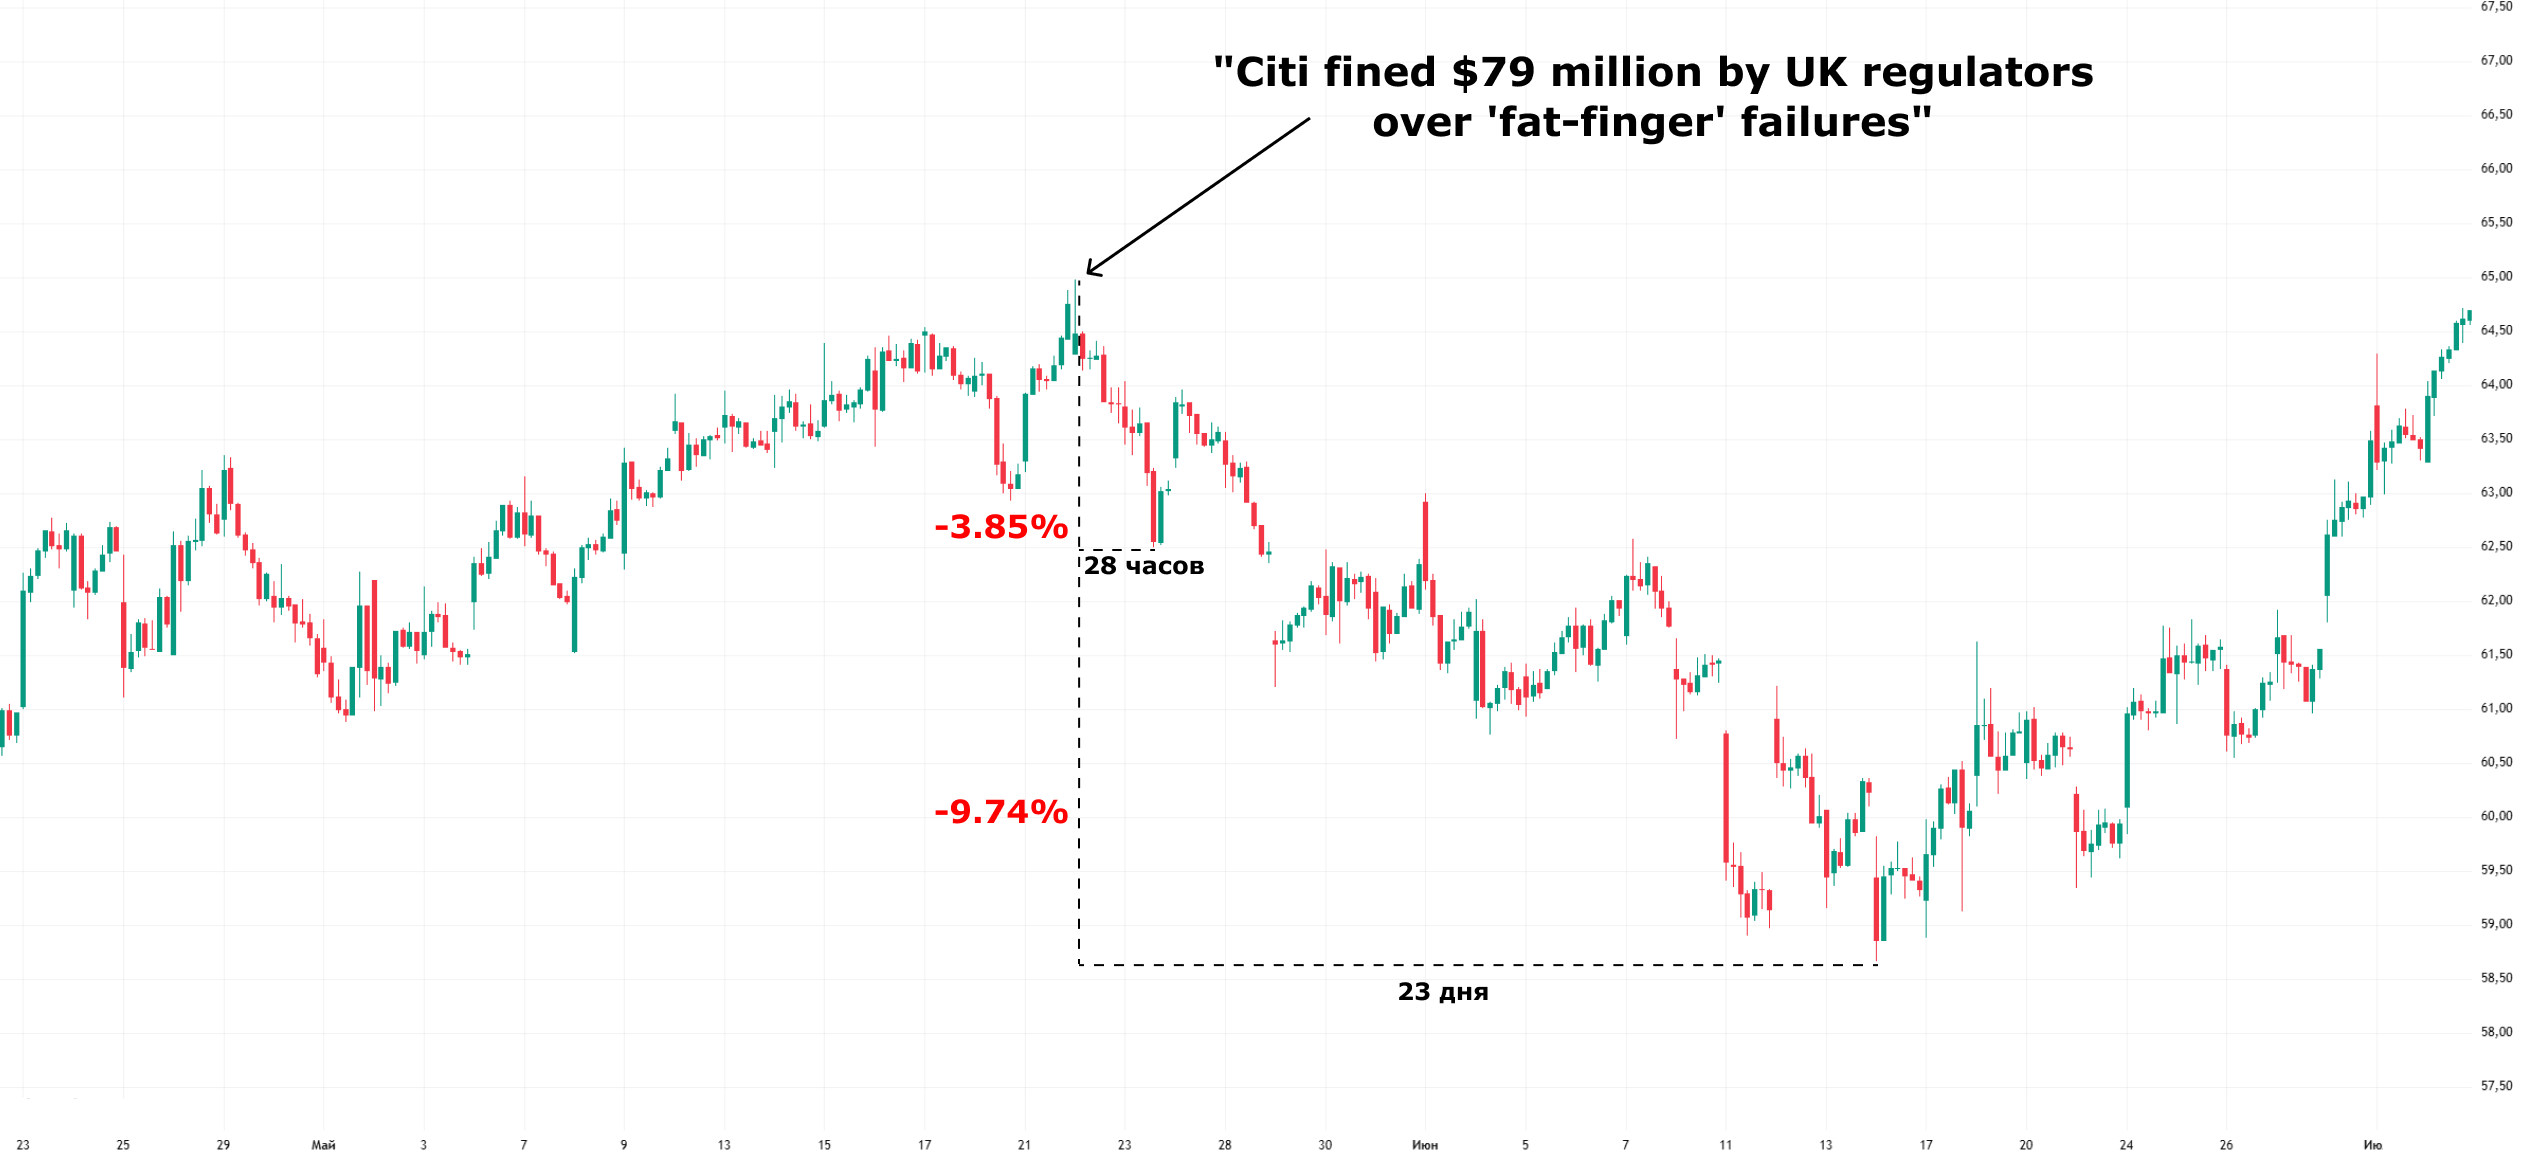
\includegraphics[width=1\linewidth]{img/citi_group.png}
    \caption{Пример падения цены акций одного из крупнейших банков США, Citi Group (C.NYSE),
    из-за обвинений в недостаточном контроле за торговыми операциями, что вызвало падение европейских акций}
    \label{fig:citi_group}
\end{figure}

Сама новостная статья от Reuters послужила сигналом для продажи актива, а на Изображении \ref{fig:citi_group} явно виден
переломный момент с резким падением цены, небольшим откатом и дальнейшей сменой глобального тренда почти на месяц.

Без FinABYSS подобные сигналы часто теряются в потоке новостей, в то время как разработанная система упрощает обнаружение
триггерных событий, посредством реализации возможности отслеживания значимых для конкретного портфеля кластеров.

Второй кейс связан с публикацией от 30 августа 2024 года о возможном отзыве лицензии и штрафе AU\$ 67 млн в отношении крупнейше
 австралийской компании по азартным играм --- The Star Entertainment Group LTD (рис. \ref{fig:star_entertainment}). Новость сообщала
 об обвинениях  в отмывании денег. Акции оказались заморожены на месяц, а при возобновлении торгов их стоимость рухнула на 55\%.

\begin{figure}[H]
    \centering
    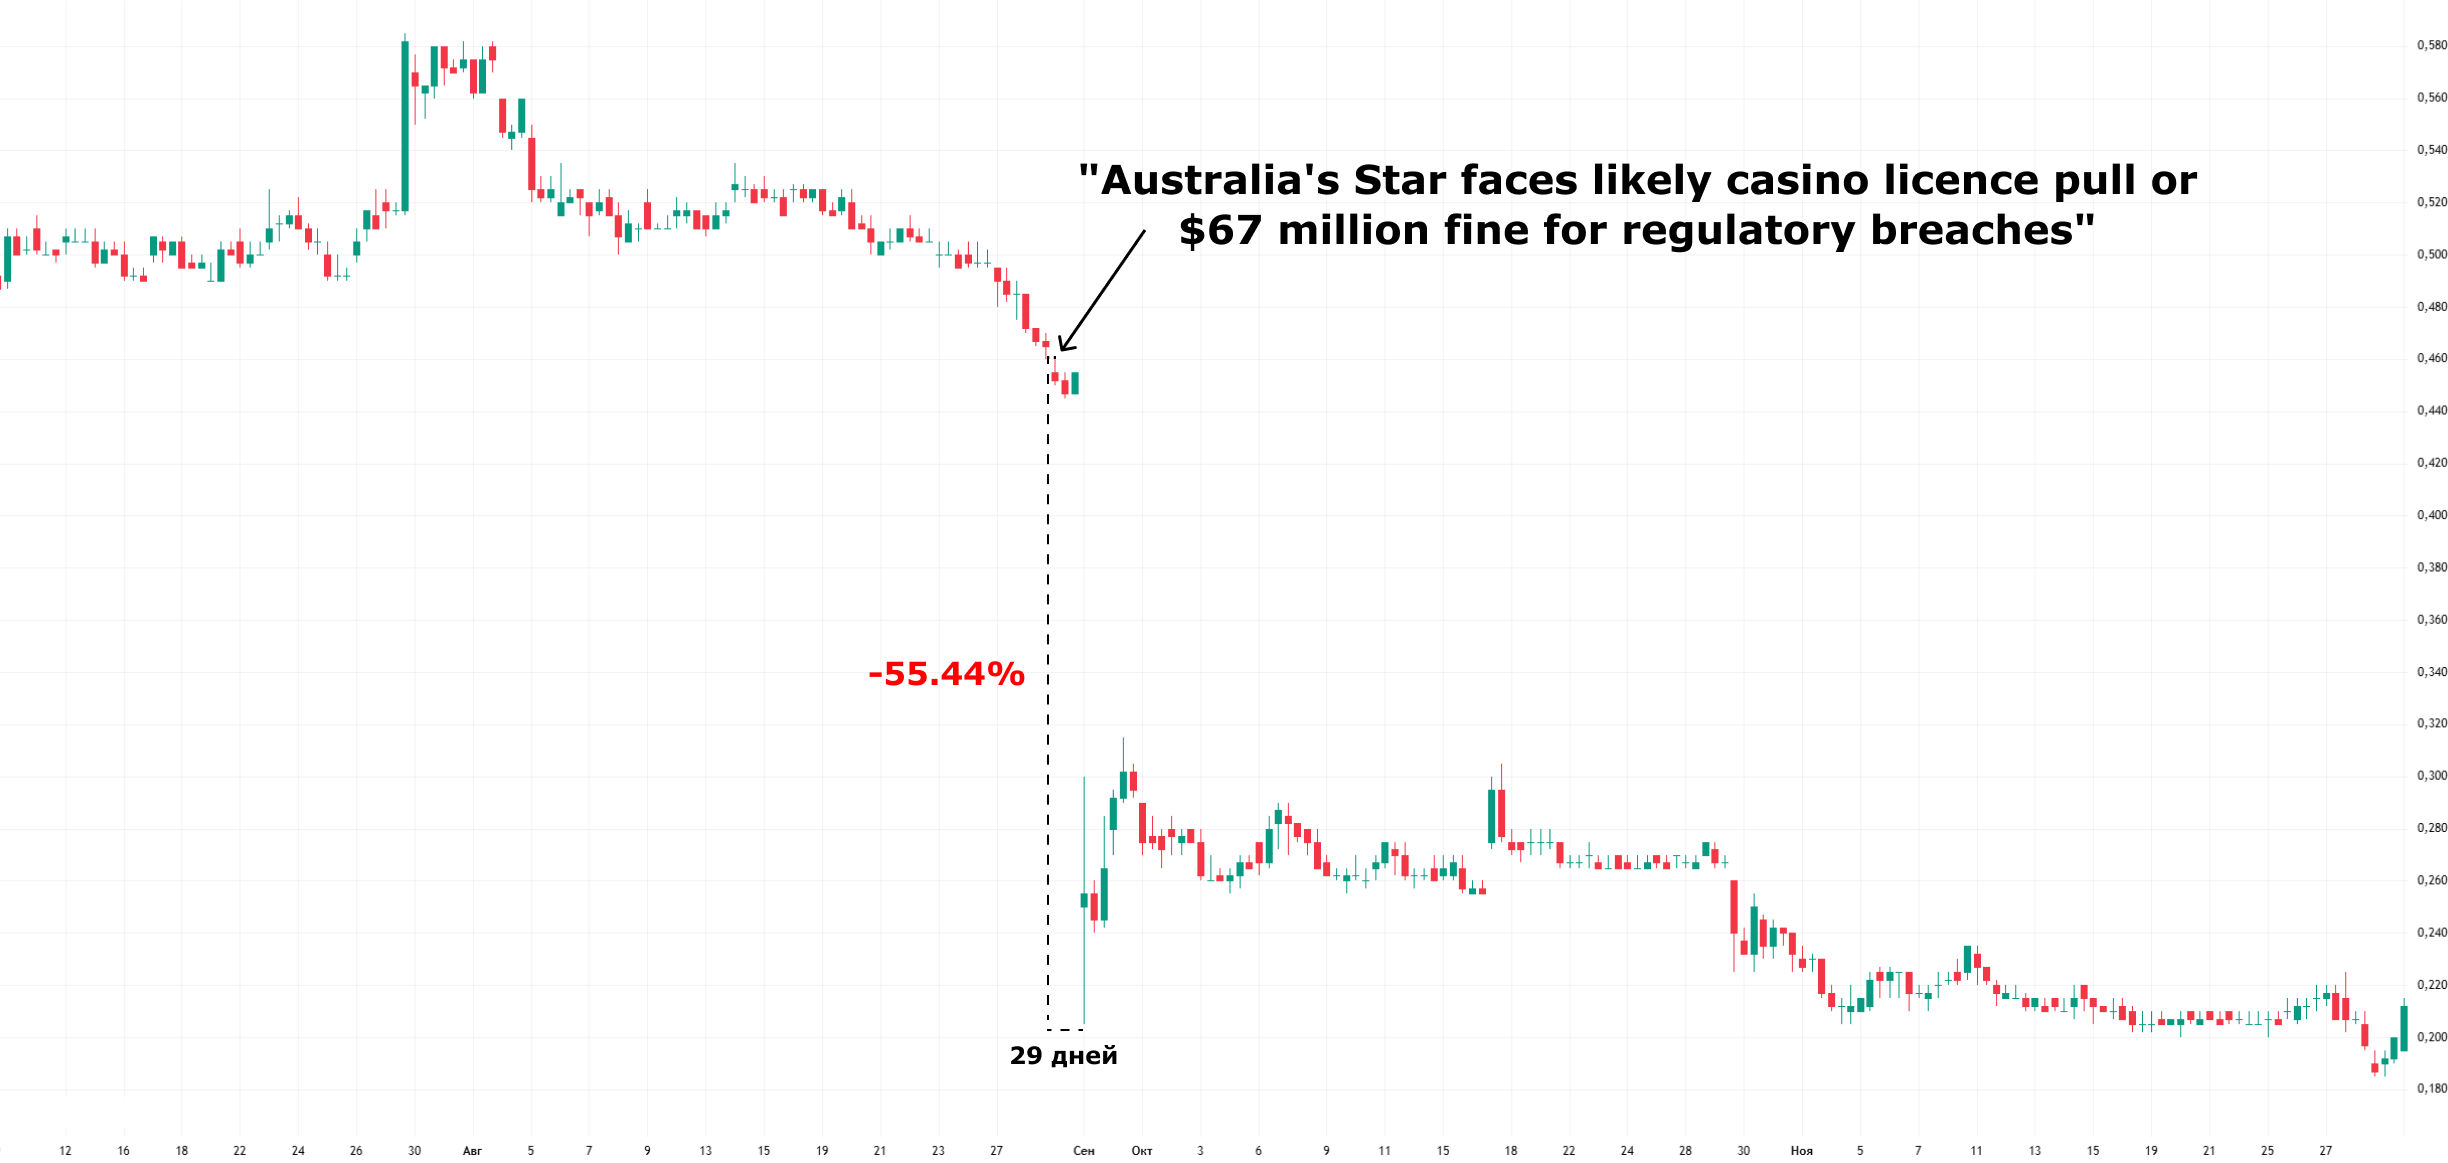
\includegraphics[width=1\linewidth]{img/star_entertainment.png}
    \caption{Пример того, как акции австралийской компании Star Entertainment Group LTD (SGR.ASX)
    обвалились и торговля ими была временно приостановлена из-за судебного разбирательства по отмыванию денег.}
    \label{fig:star_entertainment}
\end{figure}

Важно отметить, что торговля была приостановлена через сутки после публикации новости, что хоть
и является достаточным интервалом для обнаружения сигнала о продаже. Однако для рядового не вовлеченного
во внутридневную торговлю инвестора, данный сигнал весьма вероятно был бы незаметен, что привело бы
к ужасающей ситуации, когда инвестор не может продать обесценившийся актив и вынужден держать очевидный
убыток неопределенно длительный срок.

В обоих случаях, имея систему FinABYSS финансовый аналитик или инвестор мог бы одним из первых узнать
о данных инцидентах и незамедлительно отреагировать на рыночные сигналы. Простейшим способом своевременно
узнавать о триггерах является модуль активо-ориентированного отслеживания, который позволяет задать фильтры
по конкретному тикеру, источнику и тематике, чтобы получать только таргетированные сигналы.

В перспективе, после полной реализации и обучения архитектуры, предложенной в \hyperref[sec:architecture]{Разделе 3.1}, станет возможным
настройка фильтрации новостей по их сентименту, а также настройка пользовательского порога для обнаружения
значимо позитивных или негативных новостей.

Таким образом, FinABYSS выводит финансовую аналитику на совершенно новый уровень: вместо бессистемного
мониторинга СМИ и статей он получает готовые к действию алерты, визуализацию и прогнозную поддержку.
Семантическая карта уже сегодня становится неотъемлемой частью рабочего процесса, а по мере расширения
модальностей и внедрения предиктивного механизма её ценность будет лишь расти.


It is important to note that trading was halted 24 hours after the news was published, which is a sufficient
interval for a sell signal to be detected. However, for the average investor not involved in intraday trading,
this signal would very likely have been undetectable, leading to the dire situation of an investor unable to sell
a depreciating asset and forced to hold an obvious loss indefinitely.

In both cases, with FinABYSS, a financial analyst or investor would be among the first to recognize these incidents
and react immediately to market signals. The simplest way to learn about triggers in a timely manner is the asset-based
tracking module, which allows you to set filters by specific ticker, source, and topic to receive only targeted signals.

Eventually, once the architecture proposed in \hyperref[sec:architecture]{Section 3.1} is fully implemented and trained, it will be possible
to customize the filtering of news by its sentiment, as well as setting a custom threshold to detect meaningfully
positive or negative news.

FinABYSS thus takes financial analytics to a whole new level: instead of haphazard monitoring of media and articles,
it gets ready-to-action alerts, visualization, and predictive support. The semantic map is already becoming an integral
part of the workflow, and its value will only grow with the expansion of modalities and the introduction of a predictive
mechanism.